\documentclass{article}
\title{HCI Learning Diary}
\author{Candidate Number: 18512}

\usepackage{graphicx}

\begin{document}
\maketitle
\section*{Entry 1 - Initial Impressions and Concerns}

\noindent I was initially quite sceptical about the HCI module, I tend to prefer more mathematical subjects, where concepts are objective rather than subjective. I have typically done better in those kinds of modules. To be honest the first week of HCI has not put me at ease. 'Good' and 'Bad' design are concepts that are very difficult to pin down and I worry that if I am required to identify such things in an exam I will not do well.
\\\indent I thought it was interesting to see the lecture slides with pictures of old computer systems, like the punch-card computer at NASA and the old Apple Mac computer. I am interested to hear the lecturer's thoughts on punch card systems. I would also like to know if she has any ideas about programming languages in relation to HCI. Perhaps I will send an her an email.

\section*{Entry 2 - Thoughts on the Tivo Remote}

\noindent Sending an email to Kate Howland has been helped with my concerns about the module. I now seems that the subject is more objective than I realised.
\\\indent It is interesting to see the degree of relativity in our judgements about effective design. As Kate said in her email, we have no way of judging designs in a vacuum. When the punch card system was developed, or technological ability limited the degree to which the design could be user-centered.
\\\indent The Tivo remote discussed in the text-book is an interesting example. There is certainly a problem with most TV remotes. I think the minimal approach that the Tivo remote takes could be taken even further - I think a 4-way navigation button, a select button, a power button and volume buttons would be ideal. This bare minimum allows all other functionality to be managed as part of the on-screen GUI. This would eliminate the problem that reading-glasses wearers have - they require glasses to see the remote buttons but not the TV screen.
\\\indent The Tivo remote reminds me of an example of an interface with awful feedback - my freesat box at home takes far too long to respond to button presses on the remote, sometimes as much as 10 seconds. It makes you think that the press was not detected, so you press it again, and then all of a sudden, it registers both presses. If you're scrolling through the TV guide and you were trying to go down a page, this means you accidentally go down two pages, which is very frustrating.

\section*{Entry 3 - An App Review}

\noindent For my group project this week, my 'homework' was to review an existing study assistant app, with a focus on usability goals. My chosen app is 'Papyrus', a handwriting/note-taking app for android.
\\\indent \textbf{Effectiveness} - 4 stars. The pinch-to-pan/zoom feature allows you to edit writing either in fine detail, or in a less considered way.
\\\indent \textbf{Efficiency} - 1 star. While the zooming/panning is very effective, it does take a long time to actually input writing, because there is so much panning and zooming required to manipulate the page in order to be ready to enter text. Often when trying to pan \& zoom, only one finger is registered, and instead of panning or zooming, a line is drawn. You then have to press 'undo', and try again. This is frustrating and slows things down considerably.
\\\indent \textbf{Learnability} - 4 stars. Menus are very short, settings are well explained and not too extensive. The brush size/colour options are familiar and recalling how to use them is trivial.
\\\indent \textbf{Memorablity} - 4 stars. The points from learnability apply here. There is so little to learn about the app that memorising the steps to achieve tasks is trivial.
\\\indent \textbf{Safety} - 4 stars. There is a delete note/notebook confirmation which prevents accidental deletion. There are undo and redo buttons in the editor to undo mistakes. One potential (but rather unlikely) issue would be to make a mistake, and then leave the note. When you re-enter the note, you cannot undo previous changes. If this option were added, this would not be an issue.
\\\indent \textbf{Utility} - 3 stars. A good range of options relating to handwriting entry, such as brush size, colour etc. Ability to sort notes into different categories, however one note cannot be in multiple categories. The app lacks anything beyond handwriting entry - on-screen keyboard entry would be very useful due to the slowness that results from the need to pan \& zoom.
\\\indent \textbf{Summary} - Due to the inefficiency of the app's primary task, the app is effectively useless. The idea of the app is that handwriting entry is faster than using an on-screen keyboard, and therefore is a good replacement for it when speed is an issue, is completely undermined by the slowness that results from panning and zooming so often.

\section*{Entry 4 - Thoughts on the Cognitive Aspects of Interaction Design}

\noindent It is surprising to me that Miller's theory that the short term memory can hold 7 $\pm$ 2 chunks of information, has been so widely misapplied in the field of HCI. It is a mistake to apply this theory by, for example, limiting the number of options in a menu to 7, because we are not required to use our short term memory to memorise the entries in the menu - we can look at the menu as long as we like in order to decide which option to take. The fact that this theory has been so widely misapplied, I think serves as a warning when applying psychological principles to the practice of interaction design.
\\\indent I think it is actually quite difficult to find an application for Miller's theory in interaction design. It is generally the case that all the information relevant to the user's task is displayed to them by the interface of whatever it is they are interacting with, so memorisation is not required at all. Long term memory can make the use of complex interfaces with many options more efficient, in that if the user has the 'locations' of all relevant options and dialogues memorised, they can find them more quickly than if they had to search for them. However this is not related to Miller's theory as it is not to do with short-term memory.
\\\indent I thought it was interesting to see how context can affect the way we perceive things. In figure 1, taken from the lecture slides, we see that the central figure appears as the letter B when read downwards, with the context of letters context, and as the number 13 when read across, in the context of numbers.
\\\begin{center}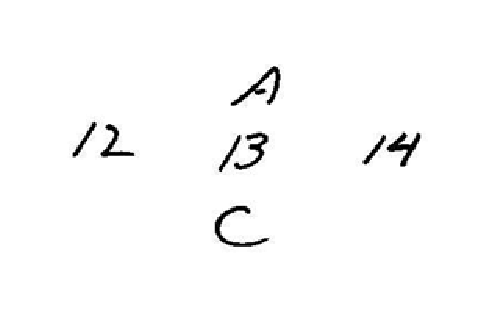
\includegraphics{context}\\\textbf{Figure 1: an example of the effects of context}\end{center}
I think this observation has significant implications for interaction design. It leads us to choose elements with less ambiguity, to prevent contexts from incorrectly giving the user the wrong idea about those elements. It also leads us to design in a way which makes good use of context - grouping elements which belong in the same context in order to make their functions clearer.

\section*{Entry 5 - User Research Methods}

\noindent This week I read an interesting article on user research methods, that I was linked to via Study Direct. The article presented an analysis of various user research methods in a fairly objective manner. According to the article, a given user research method can be thought of \& reasoned about in three different dimensions.
\\\indent The first relates to the \emph{Qualitative} and \emph{Quantitative} nature of the various research methods. Qualitative methods are useful for gaining an understanding of \emph{what} things need to change in a design, and \emph{why} they need to be changed. In contrast, Quantitative methods tend to yield more objective data. For example, a quantitative method would not be able to tell you why a particular design is good or bad, but it would be able to tell you if it is good or bad, and give you an idea of how good or bad it is, for example by comparing the average times to complete given tasks with one design versus another. Some exemplary qualitative methods are focus groups, interviews \& lab usability studies, whereas online surveys \& usage statistics collection exemplify quantitative research methods.
\\\indent The second dimension in which we can reason about user research methods is that of \emph{Behavioural} versus \emph{Attitudinal} data sources. Attitudinal sources give you information about what people say \& think, whereas behavioural sources yield information about how people actually behave, which can often conflict with attitudinal data. Attitudinal data tends to be used more heavily in marketing, as it is used to understand changes in opinions \& beliefs. Behavioural sources are typically more useful for an interaction designer, as they relate more directly to the effectiveness of a design. A/B testing, eye tracking \& usage statistics collection are typical behavioural research methods, whereas surveys, focus groups \& interviews are typical examples of attitudinal methods.
\\\indent The last dimension relates to the degree to which a user research method \emph{emulates a real-world usage scenario}. The closer a method is to a real world scenario, the more reliable the data, generally speaking. However, this is usually offset by an increase in the cost of performing the research. For example, it is very cheap, both in terms of time and money, to put together \& circulate a survey, although they do not usually yield data that tells you how people interact with a product in the real world. Performing a lab usability study, however, while highly time consuming (each participant must be observed) and expensive (participants will typically need to be paid), the data they provide very closely emulates a real world usage scenario. Ethnographic field studies \& user diaries are highly natural, and provide real-world usage information, whereas surveys \& focus groups are much more decontextualised examples, further from real world usage scenarios.

\section*{Entry 6 - Thoughts on Vim}

\noindent Vim is a text editor that has existed in various forms since the early seventies. I have been using it as my main development environment since this August, but for several months prior to this, I had been attempting to learn it, unable to switch from my previous environment - Vim is entirely reliant on commands and key combinations (it runs within the command-line and so does not have any menus etc) and so for an entirely new user to open Vim and just 'start typing' is impossible without constantly referring to documentation. And it is very painful to use any software that requires you to constantly look up how to do something. Vim is a \emph{modal} editor, it has two main modes: normal mode, in which keypresses do not enter text, but submit commands; and insert mode, where typing enters text as normal. Understanding this is a barrier for most people. However, after a couple of months, I saw patterns begin to emerge. Vim commands have two components: \textbf{motions}, which correspond to some movement of the cursor; and \textbf{actions}, which correspond to manipulation of text. Some typical motions are:
\begin{itemize}
    \item \textbf{tX} - move \textbf{t}o the next occurrence of the character \textbf{X} (this can be any character, e.g. \textbf{td} moves the cursor to the next occurrence of the character \textbf{d})
    \item \textbf{b} - move \textbf{b}ack to the beginning of the current word or previous word
    \item \textbf{\$} - move to the end of the current line
    \item \textbf{w} - move to the next \textbf{w}ord
\end{itemize}
Some common actions are:
\begin{itemize}
    \item \textbf{d} - \textbf{d}elete
    \item \textbf{y} - copy, or '\textbf{y}ank'
    \item \textbf{c} - \textbf{c}hange
\end{itemize}
The real brilliance of Vim is in the way that motions and actions are combined - they can be combined in arbitrary ways for a multitude of possible commands:
\begin{itemize}
    \item \textbf{dw} - \textbf{d}elete the next \textbf{w}ord
    \item \textbf{ct)} - \textbf{c}hange all text up \textbf{t}o the next '\textbf{)}' character
\end{itemize}
Numbers can be introduced to repeat commands:
\begin{itemize}
    \item \textbf{d2w} - \textbf{d}elete the next \textbf{2} \textbf{w}ords
\end{itemize}
I find this system to be incredibly effective, and after getting past the initial learning curve, am now much faster at editing text than I was in my previous text editor. I think it is a very elegant system, and would go so far as to say that using Vim is like speaking a language - While it is difficult when one must learn the words and grammar of the language, once a certain level of proficiency is achieved, one can begin to construct sentences of their own, that they have never seen before. I find myself doing this regularly in Vim, constructing commands that are new to me, out of motions and actions that make sense together, and finding that the desired result is achieved.
\\\indent I would say that Vim provides a level of consistency that no other interactive computer application I have used matches, and as a result is incredibly efficient and effective. I believe Vim meets the other usability goals as well - the consistency of the commands also aids in memorability \& learnability, and the sheer amount of possible commands provide excellent utility. Vim provides good security in that it prevents you from using the standard exit command (\textbf{:q}) when the file you are closing is not saved - to exit without saving, you must enter \textbf{:q!}, which you are unlikely to do mistakenly. You can also undo and redo with \textbf{u} and \textbf{CTRL-r} respectively.

\section*{Entry 7 - Prototyping}

\noindent Prototyping is useful as it allows stakeholders to gain an understanding or idea about the project. It aids in the visualisation \& reflection on the design, and is a means of communication for the design team. Prototypes can be used to explore the physical aspects of a design, such as weight, size and shape. They can give designers an indication of whether or not a design is technically possible, and 'give them a feel' for design aspects such as screen layouts, graphic design, security issues, etcetera.
\\\indent Prototype fidelity is a spectrum, from very low fidelity, such as sketches on a chalkboard, to very high fidelity, providing a close representation of the completed product. They typically start as very low fidelity, and are iteratively improved throughout the design process as problems are identified and features are added, until a high fidelity prototype is produced.
\\\indent The table below (while somewhat idealised) gives an idea of the purposes of different fidelity prototypes:
\\\\
\begin{tabular}{ | l | l | }
    \hline
    \textbf{Prototype Fidelity} & \textbf{Suited Purposes}              \\
    \hline
    Low Fidelity                & Explore different representations     \\
                                & Choose from different representations \\
                                & Test interaction \& interface style   \\
    \hline
    Mid Fidelity                & Task centered walkthroughs            \\
                                & Single task redesign                  \\
                                & Heuristic evaluation                  \\
    \hline
    High Fidelity               & Usability testing                     \\
                                & Limited field testing                 \\
    \hline
    Working Systems             & Alpha \& beta testing                 \\
    \hline
\end{tabular}\\
\\\indent Creating and testing prototypes in our project has been a very useful exercise, mostly in that it has shown me what not to do when prototyping. We started with a mid fidelity prototype, and quickly became invested in our ideas, having put a fair amount of work into them. This caused several group members were unwilling to change aspects that the other team members thought were poor. If I were to do the project again, I would start with a much lower fidelity prototype, so that ideas could be explored and discussed by the group members without the time investment of something higher fidelity, which would prevent people from being defensive about their work and unwilling to adapt.

\section*{Entry 8 - Heuristic Evaluation}

\noindent I had a read of an article posted to the study direct site this week, titled 'How to conduct a heuristic evaluation'. What I found particularly interesting were the graphs relating to the number of evaluators used. It seems that the proportion of usability problems identified by evaluators increases very quickly for the first few evaluators, and quickly levels out, such that by the time the curve reaches 15 evaluators, its gradient is almost zero. The information in the graph can be used in a cost benefit analysis, to show that the ratio of benefits to costs peaks with 5 evaluators, and after this point, the number of problems that evaluators find is sufficiently small that it is no longer cost effective to conduct evaluations. I found this very surprising - 5 seems like an incredibly small number participants. This statistic is useful - if I were planning to conduct an evaluation, I would definitely assume that more than 5 participants would be required for optimum results.

\section*{Entry 9 - Thoughts on Ubiquitous Computing}

\noindent It is interesting to consider Mark Weiser's vision of the future of computing. We have certainly not yet come close to a realisation of this vision - However I would say that smartphones \& tablets represent progress towards his idea of 'pads'. In his seminal paper, 'The Computer for the 21st Century', his description of the functionality of pads is not too far from modern day tablets. However, in contrast to today's tablets, he describes pads as 'scrap computers, analogous to scrap paper' - this could not be further from today's reality. Tablets tend to be highly personal devices, and are prized highly by their owners, and could almost be described as fashion accessories. Despite this, it is not difficult to imagine that as the cost of these devices drops, this will change, so that we might be able to 'Spread many electronic pads around on the desk, just as you spread out papers' as Weiser describes.
\\\indent I found the discussion of the appropriateness of the design principles for ubiquitous computing interesting. The image of the 'Flow Blocks' stood out to me in particular as an example of where the design principles break down.
\\\indent With objects like these flow blocks, the concept of mapping becomes less well defined. Mapping dictates that there should be a clear logical connection between controls and real world results. With the flow blocks, the control mechanism and the real world results are one and the same thing, so essentially we get mapping 'for free' with devices like this.
\\\indent Constraints also 'come for free' with the flow blocks - it is clear exactly what you cannot do with the blocks simply by their 3D shape - if you cannot fit two blocks together in a certain way, then they are not intended to be connected that way. It seems a similar rule applies for both visibility and feedback also applies. Perhaps this is because the design principles lead us to designs that mimic real world objects like chairs and paper, and so when our interfaces \emph{are} real world objects, they abide by those principles inherently. So perhaps we do need new design principles, not because the existing ones are invalid, but because they are inherent in 3D, real world interfaces, and we should instead focus our attention on design aspects that are not inherent in the nature of the interface.

\section*{Entry 10 - Elysium Guest Lecture}

\noindent It was great to hear about how the UCD principles apply in a real world scenario. I'm more interested in the programming side of things, and so while I don't think UCD will ever be the focus of my career, it will certainly be a consideration throughout. I think for this type of person, as was said in the lecture, it is very important to be aware that:
\begin{itemize}
    \item Programmers make terrible personas
    \item Programmers cannot detect design problems with their own apps
    \item Things are obvious to programmers that are not obvious to most people
\end{itemize}
These are tenets that I will try to carry through my carreer.
\\\indent It was also valuable to hear about the differences in approach to UCD for different types of company. It is important to be aware that a large company that exists to make profit for shareholders, will only take an interest in UCD as far as it is profitable - They would typically not be interested in improving user experience on products once those products no longer drive profits. Smaller companies, however, would be more likely to invest more time in UCD, and software development companies in particular will find the UCD process to be vital to their everyday work.
\\\indent As someone who finds reading difficult, I was pleased to hear that Elysium do not use traditional requirements \& design documents, but use prototypes and sketches heavily. This is a practice I think I would find both more effective and much easier. I also found it interesting to hear that the UCD principles can generalise to many aspects of business, such as person to person interaction.

\end{document}
